\section{Momenti magnetici elementari e magnetizzazione della materia: interazione con campo statico.}\linkdest{magnetizzation}

\begin{frame}{Signal from magnetized material}
%succo
\begin{align*}
&emf=-\TDof{t}\int d^3r\vec{M}(\vec{r},t)\cdot\vec{\mathcal{B}}_{rec}\\
&S\propto \frac{\gamma^3B_0^2\rho_0}{T}
\end{align*}
\end{frame}
%
\begin{wordonframe}{Magnetizzazione longitudinale all'equilibrio}
La magnetizzazione longitudinale di equilibrio \'e determinata dalla probabilit\'a di occupazione livello energetico $\exp{\exp{-\frac{\scap{m}{B}_0}{KT}}}\approx1-\frac{\scap{m}{B}_0}{KT}$: l'''eccesso'' di spin con con campo $B_0$ \'e $N\frac{\hbar\omega_0}{2KT}$. $\mu=\gamma\vec{J}$, $\gamma=\SI{1.67e8}{\rad\per\tesla\per\second}$ ([\si{\newton\meter\per\tesla}], [\si{\ampere\square\meter}]).
La magnetizzazione risultante \'e $M_0=\rho_0\frac{\gamma^2\hbar^2}{4KT}B_0$. (momento dipolo magnetico per unit\'a di volume)
\end{wordonframe}

\begin{frame}[allowframebreaks]{Equazione del moto dipolo magnetico}
\begin{columns}[T]\begin{column}{0.5\textheight}
\begin{block}{Equazione del moto (bloch0)}
\begin{align*}
&\TDy{t}{\vec{\mu}}=\gamma\vec{\mu}\wedge\vec{B}\\
&|d \mu|=\mu\sin{\theta}d \phi=\gamma\mu B\sin{\theta} dt\\
&\TDof{t}\vec{\mu}^2=0,\ \TDof{t}(\scap{\mu}{B}_0)
\end{align*}
\end{block}
%%succo
\begin{block}{Soluzioni campo B costante: precessione }
\begin{align*}
&\omega=|\TDy{t}{\phi}|=\gamma B\\
&\Rightarrow\ \phi=-\omega_0+\phi_0\\
&\mu_+(t)=\mu_x(t)+i\mu_y(t)\\
&=|\mu_+(t)|\exp{i\phi(t)}
\end{align*}
\end{block}

\end{column}\begin{column}{0.5\textheight}
\begin{block}{Momento magnetico nucleare}
\begin{columns}  \begin{column}{0.05\textwidth}\Pproton\end{column} \begin{column}{0.95\textwidth}
Rapporto giromagnetico: $\vec{\mu}=\gamma\vec{J}$, $\gamma=\SI{2.675e8}{\rad\per\second\per\tesla}$, $\gammabar=\SI{42.58}{\mega\hertz\per\tesla}$.
\end{column}  \end{columns}
\begin{align*}
&\mu_B=\frac{e\hbar}{2m_e}=\SI{9.27e-24}{\ampere\per\square\meter}\\
&\mu_B=\frac{e\hbar}{2m_n}=\SI{5.05e-27}{\ampere\per\square\meter}
\end{align*}
\end{block}
\begin{block}{Momento delle forze}
\begin{align*}
&(\vec{F}=\TDy{t}{\vec{p}})\ d \vec{F}=\vecp{J}{B}\\
&(=Id \vec{l}\wedge\vec{B})\\
&d\vec{N}=\vec{r}\wedge d \vec{F}=\vec{x}\wedge(\vecp{J}{B})
\end{align*}
\end{block}
\end{column}  \end{columns}
\end{frame}

\begin{wordonframe}{spin e dipoli magnetici}

\begin{columns}\begin{column}{0.5\textwidth}
\begin{figure}[!ht]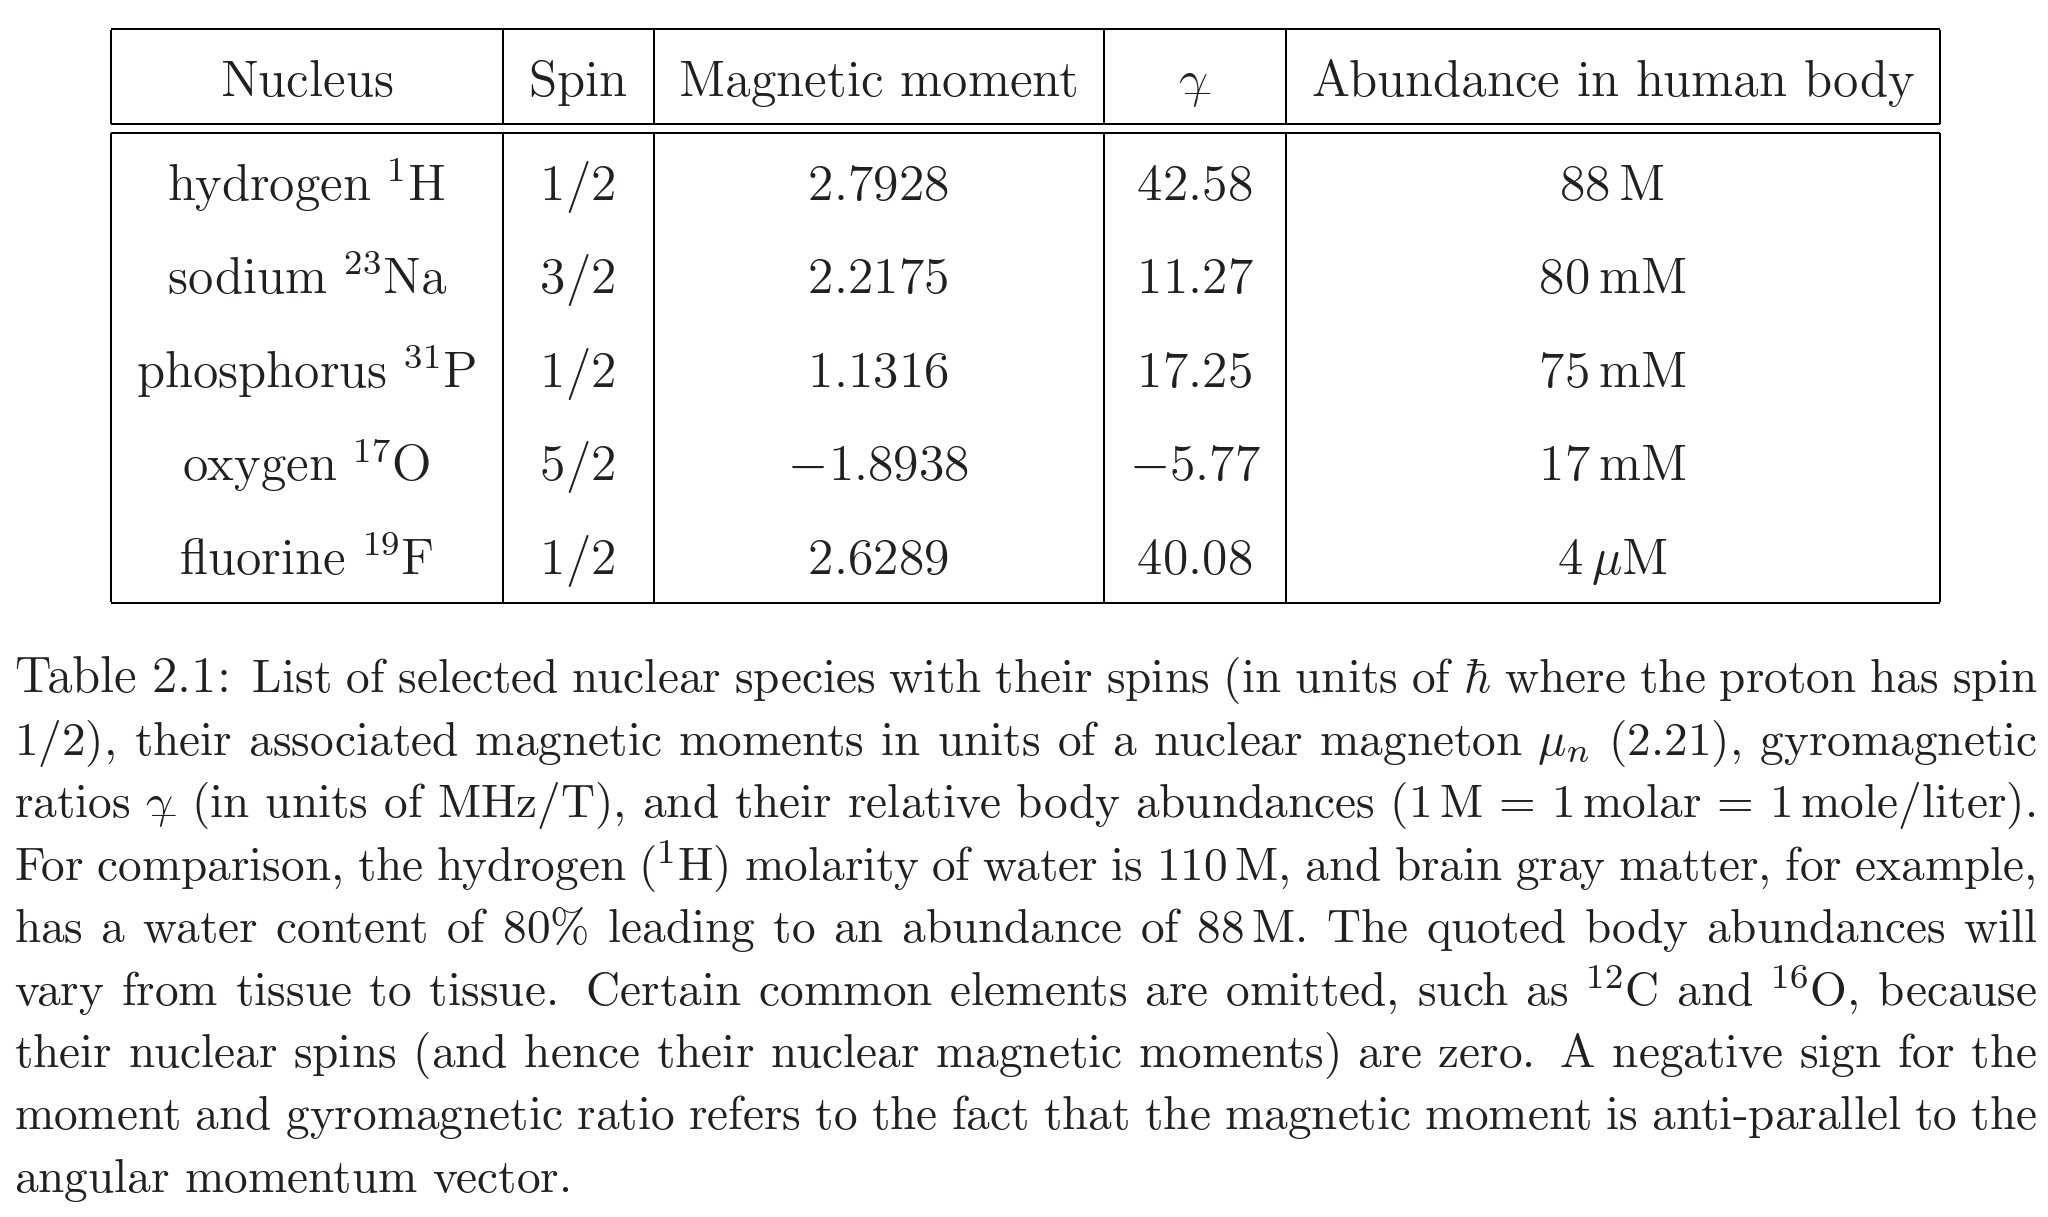
\includegraphics[trim={0cm 0cm 0 0},clip, keepaspectratio,width=0.99\textwidth]{nuclei}\label{fig:nuclei}\end{figure}
\end{column} \begin{column}{0.5\textwidth}
\begin{align*}
&\gamma=\frac{\mu}{J}\\
&\frac{\gamma_n}{2\pi g_n}=\frac{\mu_N}{h}=\SI{7.6}{\mega\hertz\per\tesla}\\
&\gamma_e=-2 \frac{e}{2m_e}\\
&\gamma_p=2.79\frac{e}{2m_p}\\
&\gamma_n=-1.91\frac{e}{2m_n}
\end{align*}
\end{column}\end{columns}
\begin{columns}  \begin{column}{0.5\textwidth}
Atomo con Z elettroni
\begin{align*}
&\vec{\mu}=-g_J \frac{e}{2m}\vec{J}\\
&g_J=\frac{3}{2}+\frac{S(S+1)-L(L+1)}{J(J+1)}
\end{align*}

\end{column} \begin{column}{0.5\textwidth}
Frequenze di Larmor: moto orbitale elettroni $\nu_L=\SI{1.4e10}{\hertz\per\tesla}$, spin elettronico $\nu_L=\SI{2.8}{\mega\hertz\per\gauss}$, spin protonico $\nu_L=\SI{4.3}{\kilo\hertz\per\gauss}$
\end{column}  \end{columns}
\end{wordonframe}

\section{Condizione di risonanza: campo trasverso $B_1$}\linkdest{resonance}

\begin{frame}[allowframebreaks]{Campo a radiofrequenza rotante}
\begin{block}{SR rotante}
\begin{align*}
&\TDy{t}{\vec{\mu}}=(\TDy{t}{\vec{\mu}})'+\vecp{\Omega}{\mu}=\gamma\vecp{\mu}{B}\\
&(\TDy{t}{\vec{\mu}})'=\gamma\vec{\mu}\wedge\vec{B}_{eff}\quad B_{eff}=\vec{B}+\frac{\vec{\Omega}}{\gamma}
\end{align*}
\end{block}
\begin{block}{EOM per campo $B_1$ a RF circolare}
\begin{equation*}
\vec{B}_1^{circ}=B_1(\hat{x}\cos{(\omega t)}-\hat{y}\sin{(\omega t)})
\end{equation*}
fermo nel riferimento rotante: $\vec{\Omega}=-\omega\hat{z}$.
\begin{align*}
&(\TDy{t}{\vec{\mu}})'=\vec{\mu}\wedge[\hat{z}'(\omega_0-\omega)+\hat{x}'\omega_1]=\gamma\vec{\mu}\wedge\vec{B}_{eff}\\
&\omega_0=\gamma B_0,\ \omega=\text{RF lab freq.},\ \omega_1=\gamma B_1
\end{align*}
\end{block}
\begin{block}{on-resonance condition}
\begin{columns}[T]
    \begin{column}{0.5\textheight}
 %%succo
    Per $\omega=\omega_0$:
\begin{align*}
&(\TDy{t}{\vec{\mu}})'=\omega_1\vec{\mu}\wedge\hat{x}'
\end{align*}
Flip-angle: $\Delta\theta=\gamma B_1\tau$.
    \end{column}
    \begin{column}{0.5\textheight}
    RF on-resonance solution
    \begin{align*}
    &\vec{\mu}(t)=R_{x'}(\phi_1(t))\vec{\mu}(0)\\
    &\phi_1(t)=\omega_1t\to\int_{t_0}^td t'\omega_1(t')
    \end{align*}
    \end{column}
\end{columns}
\end{block}
\end{frame}

\begin{wordonframe}{SR rotanti e on-resonance condition (chap 3)}
\begin{equation*}
\TDy{t}{\vec{V}}=(\TDy{t}{V})'+\vecp{\Omega}{V}
\end{equation*}
\begin{block}{Problema 3.3}

\end{block}
\end{wordonframe}

\section{Evoluzione componenti magnetizzazione longitudinale e trasversa: precessione + spin-lattice + spin-spin.}\linkdest{blocheq}

\begin{frame}[allowframebreaks]{Magnetizzazione in campo esterno: $T_1$, $T_2$. Equazione di Bloch.}
\begin{columns}[T]
\begin{column}{0.45\textheight}
\begin{block}{Magnetizzazione}
($M=\frac{1}{2}\vecp{x}{J}$)
Momento di dipolo magnetico per unit\'a di volume:
\begin{equation*}
\vec{M}=\frac{1}{V}\sum\vec{\mu}_i
\end{equation*}
V=voxel: volume dove campo magnetico omogeneo, spin hanno stessa fase.
\end{block}
\begin{block}{Dephasing due to $B_{ext}$ inhomogeneities. Spin ECHO}
%succo
$\frac{1}{T_2*}=\frac{1}{T_2}+\frac{1}{T_2}$: se domina $T_2'$ dovuto a disomogeneit\'a compo magnetico esterno $\magort{}$ pu\'o essere rifasata.
\end{block}
\end{column}
\begin{column}{0.55\textheight}
\begin{block}{Interazioni spin-lattice: $T_1$.}
%succo
\begin{align*}
&\TDy{t}{M_z}=\frac{(M_0-M_z)}{T_1}\\
&M_z(t)=M_z(0)\exp{-\frac{t}{T_1}}+M_0(1-\exp{-\frac{t}{T_1}})
\end{align*}
\end{block}
\begin{block}{Local field variation: dephasing. $T_2$}
\begin{align*}
&\TDy{t}{\magort}=(\gamma\magort{}\wedge\vec{B}_{ext})_{NR}-\frac{1}{T_2}\magort{}\\
&\magort{}(t)=\magort{}(0)\exp{-\frac{t}{T_2}}
\end{align*}
\end{block}

\begin{block}{Short/long lived pulses.}
$\Delta\omega\tau_{RF}\geq\frac{1}{4\pi}$. Short: $\Delta\omega_1\gg(\frac{1}{T_1},\frac{1}{T_2})$, ignore decay during pulse. Long: steady state.
\end{block}
\end{column}
\end{columns}
\clearpage Lorentzian shape Mz as fuction of $\omega$: lezione 1 esr
\end{frame}

\begin{wordonframe}{Rilassamento spin-lattice, spin-spin e inomogeneit\'a del campo (chap 4)}
\begin{block}{Densit\'a di energia potenziale magnetica}
Gli spin tendono ad allinearsi col campo magnetico per minimizzare la densit\'a d'energia potenziale, $U_M=-\scap{M}{B}=M_zB_0$: si hanno interazioni spin lattice.
\end{block}
Legge di Curie: $M_0=C\frac{B_0}{T}$,valore di equilibrio.
\begin{block}{Evoluzione $M_z$, inizio arbitrario}
\begin{align*}
&M_z(t)=M_z(0)\exp{-\frac{t}{T_1}}+M_0(1-\exp{-\frac{t}{T_1}})\\
&0\to t_0,\ t\to t-t_0
\end{align*}
\end{block}
\end{wordonframe}

\begin{frame}{Equazione di Bloch}
%succo
    \begin{equation*}
        \TDy{t}{\vec{M}}=\gamma\vec{M}\wedge\vec{B}_{ext}+\frac{1}{T_1}(M_0-M_z)\hat{z}-\frac{1}{T_2}\magort{}
    \end{equation*}
    soluzioni:
    \begin{align*}
&M_x(t)=\exp{-\frac{t}{T_2}}(M_x(0)\sin{(\omega_0t)}+M_y(0)\cos{(\omega_0t)})\\
&M_y(t)=\exp{-\frac{t}{T_2}}(M_y(0)\cos{(\omega_0t)}-M_x(0)\sin{(\omega_0 t)})\\
&M_z(t)=M_z(0)\exp{-\frac{t}{T_1}}+M_0(1-\exp{-\frac{t}{T_1}})\\
&M_+(t)=\exp{-i\omega_0t-t/T_2}M_+(0)\to|M_+(t)|\exp{i\phi(t)}
    \end{align*}
    Per $\vec{B}_{ext}=B_0\hat{z}+B_1\hat{x}$, le equazioni di Bloch sono, con $\Delta\omega=\omega_0-\omega$:
    \begin{align*}
&(\dot{M}_{z'})'=-\omega_1M{y'}+\frac{M_0-M_z}{T_1}\\
&(\dot{M}_{x'})'=\Delta\omega M_{y'}-\frac{M_{x'}}{T_2}\\
&(\dot{M}_{y'})'=-\Delta\omega M_{x'}+\omega_1M_z-\frac{\omega M_{y'}}{T_2}
    \end{align*}
\end{frame}

\begin{wordonframe}{Regimi di applicazione}
\begin{itemize}
    \item $|H_1|\ll|H_0|$
    \item Ehrenfest adiabaticity: $\vec{H}$ and $\vec{M}$ formano angolo costante: How slowly we must change $\vec{H}$ direction so that $\vec{M}$ preserve its angle (preserving its interaction energy)? If $\vec{\Omega}$ is the rotation of $\vec{H}$ in rotating frame with $\vec{H}$
    \begin{equation*}
        (d/dt)'\vec{M}=(\gamma\vec{H}-\Omega)\wedge\vec{M}
    \end{equation*}
    quindi $\Omega\ll\gamma\vec{H}$
    \item Adiabaticity in rotating frame. We take for $\vec{H}=\hat{x}H_1\cos{\omega t}+\hat{y}H_1\sin{\omega t}+\hat{z}H_0$ Adiabatic passage through resonance $\omega=\omega_0=\gamma H_0$ (slowly sweep of $\omega$ through $\omega_0=\gamma H_0$). Defining effective field $\vec{H}_e=\vec{H}-\vec{\omega}/\gamma$. $\vec{M}=\vec{M}_0=\chi_0\vec{H}_0$ pointing along $\vec{H}_0$ and approx along $\vec{H}_e$ ($H_1\ll H_0$, $\omega\ll\gamma H_0$): initial motion is a precession of $\vec{M}$ around $\vec{H}_e$ viewed from rotating frame.
    How slowly we must change $\vec{H}_e$ in order $\vec{M}$ to follow?
    Magnetic field turn impercettible during period of Larmor precession about it:
    \begin{equation*}
    \invers{H}_1|(d/dt)(\vec{H}_0-\vec{\omega}/\gamma)|\ll\gamma H_1
    \end{equation*}
    \item rapid passage. Slowest precession in rotating frame when $\gamma\vec{H}_e=\gamma\vec{H}_1$: se $1/T_1$ or $1/T_2$ exceed $\gamma H_1$ relaxation processes cause $\vec{M}$ to decay, $1/T_2\ll\gamma H_1$. ($1/T_1\leq1/T_2$)
    \item Slow passage. Steady state condition $\TDy{t}{M_z}=0$
    \end{itemize}
\end{wordonframe}

\begin{frame}{Soluzione equazioni di Bloch: condizioni stazionarie}
    \begin{columns}[T]
    \begin{column}{0.5\textwidth}
    \begin{align*}
    &\PDy{t}{M_x}=\PDy{t}{u}=0=\frac{-u}{T_2}+v\Delta\omega\\
    &\PDy{t}{M_y}=\PDy{t}{v}=0=\frac{-v}{T_2}-u\Delta\omega-\omega_1M_z\\
    &\PDy{t}{M_z}=0=\omega_1v+\frac{M_z-M_0}{T_1}\\
    \end{align*}
    con $\Delta\omega=\omega-\omega_0$. Soluzioni:
    \begin{align*}
    &u=M_0\frac{\omega_1\Delta\omega T_2^2}{1+(T_2\Delta\omega)^2+\omega_1^2T_1T_2}\\
    &u=M_0\frac{\omega_1T_2}{1+(T_2\Delta\omega)^2+\omega_1^2T_1T_2}\\
    &M_z=M_0\frac{1+(T_2\Delta\omega)^2}{1+(T_2\Delta\omega)^2+\omega_1^2T_1T_2}\\
    \end{align*}
    \end{column}
    \begin{column}{0.5\textwidth}
    \begin{figure}
        \centering
        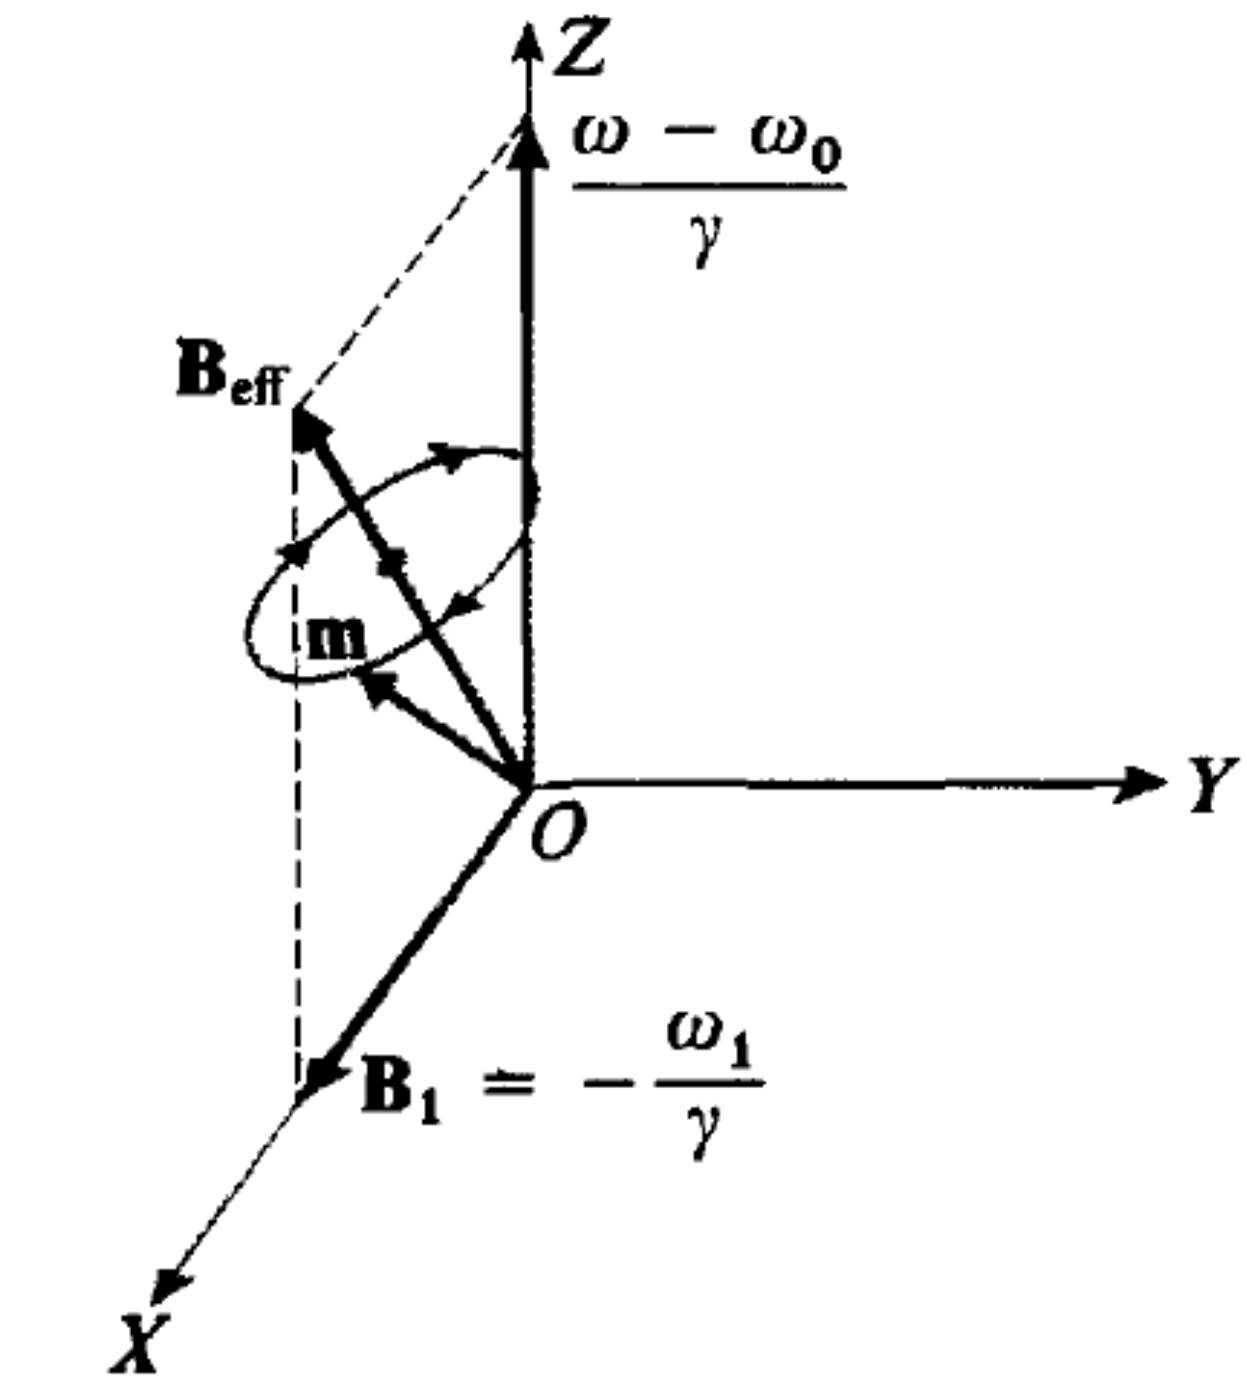
\includegraphics{MBrotCW}
        \label{fig:MBrotCW}
    \end{figure}
    Nel riferimento del Lab la magnetizzazione ruota con velocit\'a angolare costante:
    \begin{align*}
    &M_x=u\cos{\omega t}-v\sin{\omega t}=\sqrt{u^2+v^2}\cos{\omega t-\phi}\\
    &M_y=u\cos{\omega t}+v\sin{\omega t}=\sqrt{u^2+v^2}\sin{\omega t-\phi}\\
    &M_z=M_z
    \end{align*}
    Effetti del campo rotante
    \begin{itemize}
        \item Diminuzione componente $M_z$
        \item Magnetizzazione trasversa rotante con $B_1$ con ritardo $\phi$ rispetto a $B_1$: Il campo rotante compie lavoro positivo e l'energia corrispondente \'e assorbita dal mezzo.
    \end{itemize}
    \end{column}
    \end{columns}
\end{frame}

\begin{frame}{Importanza }
    
\end{frame}

\section{Tipi di rilassamento}

\begin{frame}{Magnetizzazione: popolazione livelli e coerenza}
\begin{columns}[T]
\begin{column}{0.5\textwidth}
\begin{itemize}
\item RF: Coherence excitation ($\pi/2|_x$, $\pi|_x$ inversion of population.
\item $B_0$: Different population of Zeeman splitted levels in thermal equilibrium.
\end{itemize}
\end{column}
\begin{column}{0.5\textwidth}
\begin{block}{Spontaneous/induced emission in system of spin}

\end{block}
\end{column}
\end{columns}
\end{frame}

